\section{Exercise seven}

A system comprising five modules (A, B, C, D, and E) is designed to function properly under the following conditions: either modules A or B operate correctly, and concurrently modules C and D operate correctly, or alternatively, module E operates correctly.
\begin{enumerate}
    \item Draw the reliability block diagram of the system.
    \item Find the expression for the reliability of the system.
    \item Given that the mean time to failure for modules A and B is 3412 hours, and for modules C, D, and E is 1245 hours, we aim to calculate the reliability of the system after 1 month.
\end{enumerate}

\subsection*{Solution}
\begin{enumerate}
    \item The reliability block diagram of the system is depicted below:
        \begin{figure}[H]
            \centering
            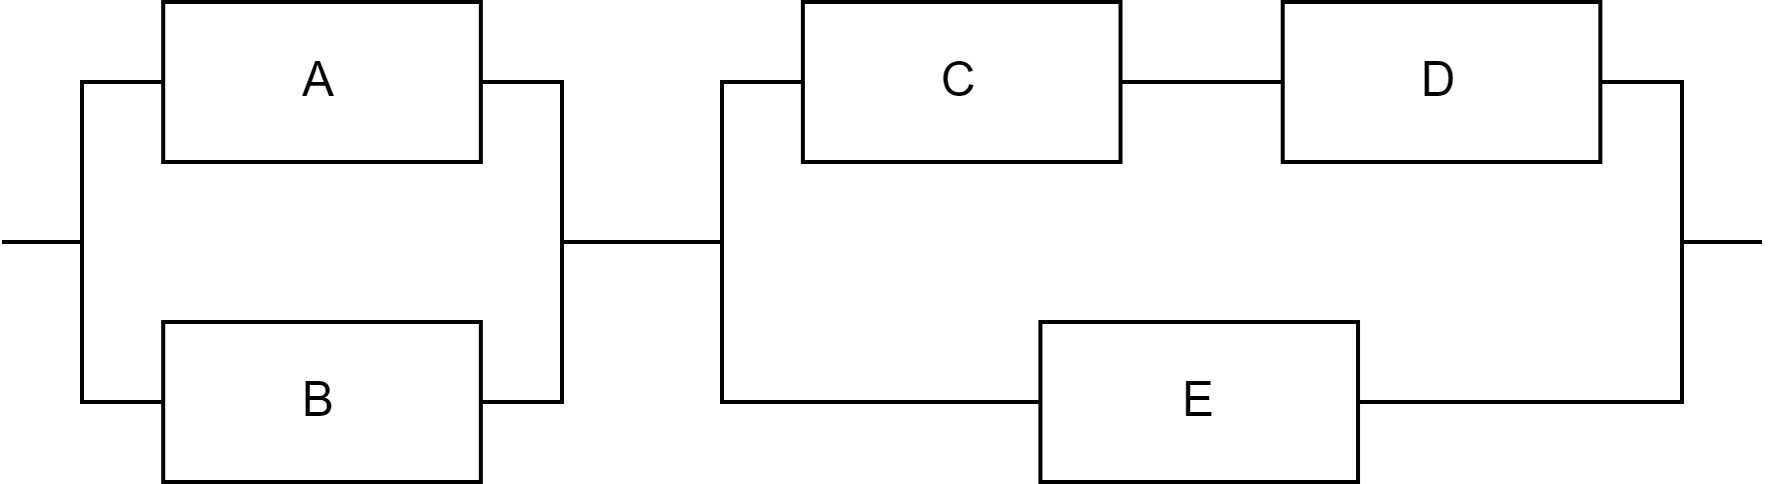
\includegraphics[width=0.6\linewidth]{images/rbd.png}
        \end{figure}
    \item The blocks A and B are in parallel, hence the total reliability is computed as:
        \[R_{\text{AB}}=1-\left(1-R_\text{A}\right)\left(1-R_\text{B}\right)\]
        The blocks C and D are in series, therefore the total reliability is:
        \[R_{\text{CD}}=R_\text{C}R_\text{D}\]
        Now, with the new block CD in parallel with E, the reliability becomes:
        \[R_{\text{CDE}}=1-\left(1-R_\text{CD}\right)\left(1-R_\text{E}\right)\]
        Finally, the entire system's reliability is the product of the reliabilities of blocks AB and CDE:
        \[R_{s}=\left[1-\left(1-R_\text{A}\right)\left(1-R_\text{B}\right)\right]\left[1-\left(1-R_\text{CD}\right)\left(1-R_\text{E}\right)\right]\]
    \item We can compute the monthly mean time to failures:
        \[\text{MTTF}_{\text{A}}=\text{MTTF}_{\text{B}}=4,74 \text{ months}\]
        \[\text{MTTF}_{\text{C}}=\text{MTTF}_{\text{D}}=\text{MTTF}_{\text{E}}=1,73 \text{ months}\]
        The monthly failure rates are the inverses of the mean time to failures:
        \[\lambda_{\text{A}}=\lambda_{\text{B}}=\dfrac{1}{4,74 \text{ months}}=0.21\]
        \[\lambda_{\text{C}}=\lambda_{\text{D}}=\lambda_{\text{E}}=\dfrac{1}{1,73 \text{ months}}=0.578\]
        We can now compute the reliability of each block:
        \[R_{\text{A}}(1)=R_{\text{B}}(1)=e^{-\lambda t}=e^{-1\cdot 0.21}=0.81\]
        \[R_{\text{B}}(1)=R_{\text{C}}(1)=R_{\text{D}}(1)=e^{-\lambda t}=e^{-1\cdot 0.578}=0.56\]
        From the previously derived formula, we find:
        \[R_{s}(1)=\left[1-\left(1-R_\text{A}(1)\right)\left(1-R_\text{B}(1)\right)\right]\left[1-\left(1-R_\text{CD}(1)\right)\left(1-R_\text{E}(1)\right)\right]=0.67\]
        Specifically, we have:
        \begin{itemize}
            \item $R_{\text{AB}}=1-\left(1-R_\text{A}\right)\left(1-R_\text{B}\right)=0.96$.
            \item $R_{\text{CD}}=R_\text{C}R_\text{D}=0.31$.
            \item $R_{\text{CDE}}=1-\left(1-R_\text{CD}\right)\left(1-R_\text{E}\right)=0.70$.
        \end{itemize}
\end{enumerate}